% Sprint 0
\chapter{Sprint 0}

\section{Introduction}
Ce chapitre présente le \textbf{Sprint 0}, 
qui marque la phase initiale de la réalisation de notre projet.
Le \textbf{Sprint 0} est une étape cruciale où nous posons les fondations du projet en identifiant les acteurs clés, 
en capturant les besoins fonctionnels et non fonctionnels,
et en définissant la méthodologie de travail qui guidera le développement. Cette phase permet de clarifier les objectifs,
les attentes et les contraintes du projet, 
tout en établissant un cadre de travail structuré pour les étapes ultérieures.


\section{Capture des besoins}
\subsection{Identification des acteurs}

Dans un premier temps, nous identifions les acteurs du système, c'est-à-dire les entités externes qui interagiront avec l'application. Ces acteurs jouent un rôle central dans la définition des fonctionnalités et des services que le système doit fournir.
\begin{table}[H]
    \centering
    \renewcommand{\arraystretch}{1.3}
    \begin{tabular}{| m{3cm} | m{7cm} |}
        \hline
        \textbf{Acteur} & \textbf{Description} \\
        \hline
        \textbf{Médecin} & Consulte les données des patients, reçoit les alertes critiques et valide les actions nécessaires. \\
        \hline
        \textbf{Infirmier(ère)} & Surveille les patients, reçoit les alertes en fonction de ses horaires et prend des mesures immédiates. \\
        \hline
        \textbf{Administrateur du Système} & Gère les utilisateurs, configure les seuils d'alerte et assure le bon fonctionnement du système. \\
        \hline
        \textbf{Moniteur de Signes Vitaux} & Source de données : envoie des informations vitales via API ou caméra. \\
        \hline
        \textbf{Caméra} & Capturent les écrans des machines et les transmet pour analyse. \\
        \hline
    \end{tabular}
    \caption{Acteurs du système et leurs rôles}
\end{table}

\subsection{Besoins fonctionnels et non fonctionnels}
Cette section détaille les besoins fonctionnels et non fonctionnels du système, qui reflètent les exigences des utilisateurs ainsi que les contraintes techniques à respecter.

\subsection*{Besoins Fonctionnels}

Les besoins fonctionnels décrivent les fonctionnalités attendues du système :

\begin{itemize}
    \item \textbf{Collecte des données} : Le système doit être capable de collecter des données en temps réel à partir des moniteurs de signes vitaux et des caméras.
    \item \textbf{Détection et reconnaissance des valeurs vitales} : Utilisation de l'OCR pour extraire les valeurs vitales à partir des images capturées.
    \item \textbf{Génération et gestion des alertes} : Le système doit déclencher des alertes en fonction des seuils définis et les acheminer au personnel médical concerné.
    \item \textbf{Affichage des données} : Une interface web et mobile permettant aux médecins et infirmiers d’accéder aux données patient.
    \item \textbf{Authentification et gestion des utilisateurs} : Gestion des rôles et permissions des utilisateurs (administrateurs, médecins, infirmiers).
    \item \textbf{Notifications} : Envoi d’alertes par e-mail, SMS ou notifications push via Firebase Cloud Messaging (FCM).
    \item \textbf{Stockage et historique des données} : Enregistrement des valeurs mesurées et des alertes pour analyse et suivi.
\end{itemize}

\subsection*{Besoins Non Fonctionnels}

Les besoins non fonctionnels définissent les contraintes techniques et de performance du système :

\begin{itemize}
    \item \textbf{Disponibilité} : Le système doit être accessible 24/7 avec une tolérance aux pannes minimale.
    \item \textbf{Sécurité} : Protection des données médicales via chiffrement et authentification sécurisée.
    \item \textbf{Interopérabilité} : Compatibilité avec différents modèles de moniteurs (Mindray, Edan) et support des standards HL7.
    \item \textbf{Scalabilité} : Capacité à gérer une augmentation du nombre de patients et d’appareils connectés.
    \item \textbf{Temps de réponse} : Le traitement des alertes doit être instantané pour garantir la réactivité du personnel médical.
    \item \textbf{Conformité} : Respect des réglementations médicales.
\end{itemize}
 




\section{Pilotage du projet avec Scrum}
Le projet sera géré selon la méthodologie \textbf{Scrum}, favorisant une approche agile avec des cycles itératifs appelés \textbf{sprints}. Le \textbf{Product Owner}, l’\textbf{équipe de développement} et le \textbf{Scrum Master} collaboreront pour assurer une livraison progressive des fonctionnalités clés.

\subsection*{Acteurs Scrum et Missions}
\begin{longtable}{|m{3cm}|m{8cm}|m{2cm}|}
\hline
\textbf{Rôle} & \textbf{Mission} & \textbf{Acteur} \\
\hline
\endfirsthead
\hline
\textbf{Rôle} & \textbf{Mission} & \textbf{Acteur} \\
\hline
\endhead
% \hline
\endfoot
Product Owner & 
- Définir et prioriser les fonctionnalités du produit (Product Backlog). \newline
- Assurer que l'équipe travaille sur les fonctionnalités les plus importantes. \newline
- Valider les livrables à la fin de chaque sprint. &
Pr Ammeri Charfeddine \\
\hline
Équipe de Développement & 
- Concevoir, développer et tester les fonctionnalités du produit. \newline
- Participer aux réunions de planification et de revue de sprint. \newline
- Assurer la qualité du code et des livrables. &
Zaibi Racha \\
\hline
Scrum Master & 
- Faciliter les réunions Scrum (Daily Stand-up, Sprint Planning, Sprint Review, Retrospective). \newline
- Supprimer les obstacles qui empêchent l'équipe de progresser. \newline
- Assurer que l'équipe suit les principes Scrum. &
Ouni Ghada\\
\hline
\caption{Acteurs du projet} 
\end{longtable}

\subsection*{Organisation du Backlog}
Le \textbf{Product Backlog} regroupe l’ensemble des fonctionnalités à développer pour le système. Chacune est formulée sous forme de \textit{User Story}, garantissant une approche centrée sur l’utilisateur.

Chaque fonctionnalité sera développée et livrée en plusieurs \textbf{sprints}, selon les priorités établies par le \textit{Product Owner}. Elles sont classées selon la méthode \textbf{MoSCoW}, qui définit les niveaux de priorité pour chaque tâche.

\section*{Backlog du Projet}
% Le \textbf{Backlog} est un élément central de la méthodologie \textbf{Scrum}. Il regroupe toutes les spécifications fonctionnelles et techniques du produit.

\begin{longtable}{|c|p{9cm}|c|}
    \hline
    \textbf{ID} & \textbf{Tâche} & \textbf{Priority} \\
    \hline
    \endfirsthead
    \hline
    \textbf{ID} & \textbf{Tâche} & \textbf{Priority} \\
    \hline
    \endhead
    % \hline
    \endfoot
    M-01 & Collecte des données en temps réel à partir des moniteurs Mindray via API/HL7. & M \\
    \hline
    M-02 & Détection et reconnaissance des valeurs vitales via OCR pour les machines anciennes. & M \\
    \hline
    M-03 & Génération et gestion des alertes en fonction des seuils prédéfinis. & M \\
    \hline
    M-04 & Envoi d’alertes aux médecins et infirmiers via notifications push (FCM) et e-mail. & M \\
    \hline
    M-05 & Interface web et mobile pour visualiser les données des patients et gérer les alertes. & M \\
    \hline
    M-06 & Authentification et gestion des utilisateurs (médecins, infirmiers, administrateurs). & M \\
    \hline
    M-07 & Stockage et historique des données pour analyse et suivi. & M \\
    \hline
    M-08 & Conformité aux réglementations médicales (sécurité des données, chiffrement). & M \\
    \hline
    M-09 & Tests de validation de la collecte de données (comparaison entre API et OCR). & M \\
    \hline
    S-01 & Intégration avec d’autres modèles de moniteurs (Edan, etc.). & S \\
    \hline
    S-02 & Configuration des seuils d’alerte personnalisés par patient ou par bloc. & S \\
    \hline
    S-03 & Gestion des horaires de filtrage des alertes pour le personnel médical. & S \\
    \hline
    S-04 & Interface d’administration pour configurer les seuils d’alerte et gérer les utilisateurs. & S \\
    \hline
    S-05 & Notifications SMS en plus des notifications push et e-mail. & S \\
    \hline
    S-06 & Scalabilité du système pour gérer un nombre croissant de patients et d’appareils. & S \\
    \hline
    C-01 & Intégration avec des systèmes tiers (IQ Messenger SmartApp, Xchart.com). & C \\
    \hline
    C-02 & Analyse prédictive des données pour anticiper les alertes critiques. & C \\
    \hline
    C-03 & Interface mobile avancée avec des graphiques interactifs pour les données des patients. & C \\
    \hline
    C-04 & Support multilingue pour l’interface utilisateur. & C \\
    \hline
    C-05 & Gestion des alertes par priorité (critique, moyen, faible). & C \\
    \hline
    C-06 & Historique des alertes avec possibilité de filtrage par date, patient, ou type d’alerte. & C \\
    \hline
    % W-01 & Intégration avec des systèmes de gestion hospitalière (HIS) tiers. &W \\
    % \hline
    % W-02 & Déploiement du système dans plusieurs hôpitaux ou centres médicaux. &W \\
    % \hline
    % W-03 & Analyse avancée des données avec intelligence artificielle pour le diagnostic médical. &W \\
    % \hline
    % W-04 & Support pour d’autres langues de programmation ou frameworks non prévus initialement. &W \\
    % \hline
    % W-05 & Développement d’une application desktop en plus des interfaces web et mobile. &W \\
    % \hline
\caption{Backlog du Projet avec Priorités MoSCoW} 
\end{longtable}
\section*{Clé des Priorités MoSCoW}
\begin{itemize}
    \item \textbf{M (Must)} : Tâches critiques nécessaires au bon fonctionnement du système.
    \item \textbf{S (Should)} : Tâches importantes qui apportent une valeur significative mais ne sont pas essentielles pour la première version.
    \item \textbf{C (Could)} : Fonctionnalités optionnelles pouvant être ajoutées si le temps et les ressources le permettent.
    \item \textbf{W (Won't Have)} : Tâches hors du périmètre de la phase actuelle du projet.
\end{itemize}

\subsection{Diagramme des cas d’utilisation global}
\begin{figure}[H]
    \centering
    \begin{minipage}{1\textwidth}
        \centering
        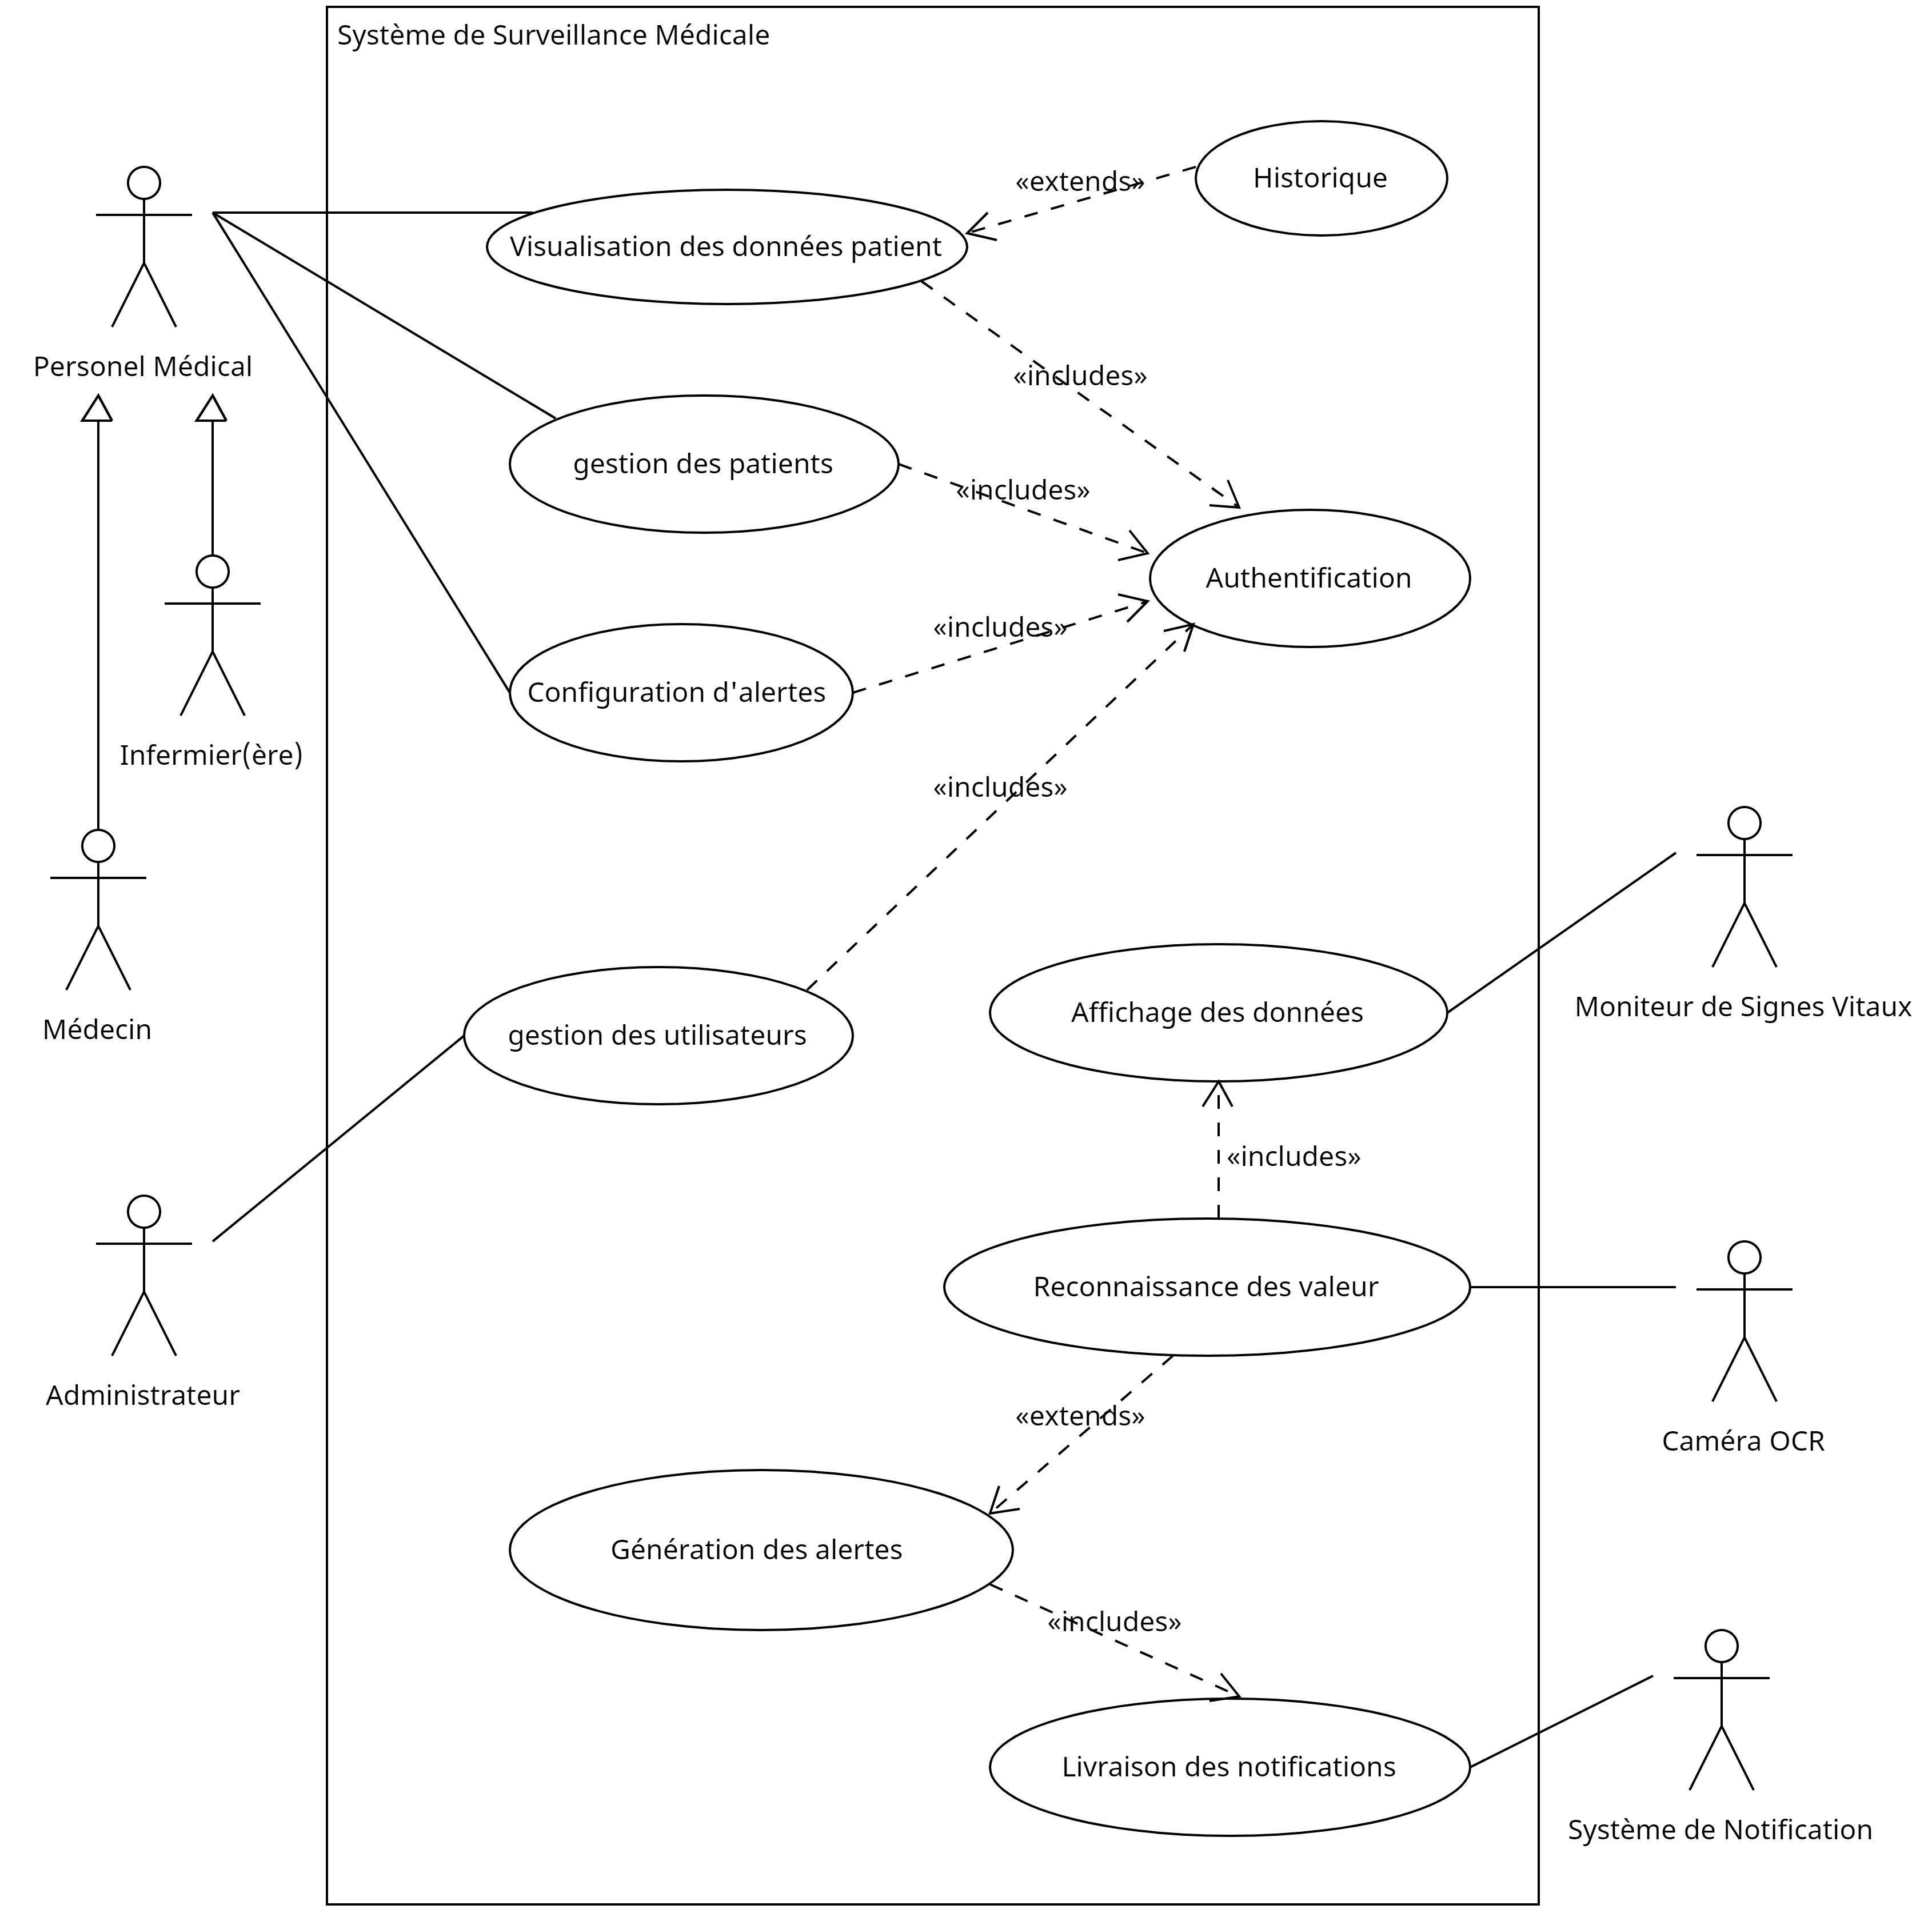
\includegraphics[width=\linewidth]{chapter2/sections/diagrams/use_case.png}
        \caption{Diagramme des cas d’utilisation global}
    \end{minipage}
\end{figure}
\subsection{Planification des sprints}
Une fois le backlog du produit finalisé, nous avons organisé la réunion de planification de sprint. L'objectif de cette réunion était de construire le backlog de sprint en se basant sur le backlog de produit défini par le Product Owner. À l'issue de cette réunion, nous avons identifié les durées prévisionnelles du travail à effectuer pour chaque sprint. Pour ce projet, nous avons divisé le travail en deux releases. La première release contient un seul sprint d'une durée de 2 semaines, tandis que la deuxième release est composée de deux sprints, chacun d'une durée de 3 semaines. La figure 2.2 illustre la répartition des sprints pour notre système.

Décrivez le plan des sprints :

\begin{itemize}
    \item \textbf{Sprint 1 : Collecte de données basée sur caméra}
    \begin{itemize}
        \item \textbf{Objectif} : Mettre en place un système de collecte de données à partir des machines anciennes en utilisant des caméras et des techniques de reconnaissance optique de caractères (OCR).
        \item \textbf{Deliverables} :
            \begin{itemize}
                \item Intégration de la caméra avec le système.
                \item Détection et extraction des valeurs vitales via OCR.
                \item Validation des données collectées par rapport aux données réelles.
            \end{itemize}
        \item \textbf{Durée} : 2 semaines.
        \item \textbf{Tâches clés} :
            \begin{itemize}
                \item Configuration des caméras et des logiciels OCR (OpenCV, Tesseract).
                \item Développement du pipeline de traitement d'images.
                \item Tests de validation des données collectées.
            \end{itemize}
        \item \textbf{Risques} : 
            \begin{itemize}
                \item Mauvaise qualité d'image affectant la précision de l'OCR.
                \item Solution : Utilisation de caméras haute résolution et prétraitement des images.
            \end{itemize}
    \end{itemize}

    \item \textbf{Sprint 2 : Collecte de données à partir des moniteurs Mindray}
    \begin{itemize}
        \item \textbf{Objectif} : Intégrer les moniteurs Mindray pour collecter des données en temps réel via des API ou des protocoles HL7.
        \item \textbf{Deliverables} :
            \begin{itemize}
                \item Connexion des moniteurs Mindray au système central.
                \item Collecte et stockage des données en temps réel.
                \item Validation de la collecte de données via API/HL7.
            \end{itemize}
        \item \textbf{Durée} : 3 semaines.
        \item \textbf{Tâches clés} :
            \begin{itemize}
                \item Configuration des API ou des protocoles HL7 pour les moniteurs Mindray.
                \item Développement du backend pour la collecte et le stockage des données.
                \item Tests de validation des données collectées.
            \end{itemize}
        \item \textbf{Dépendances} : Les données collectées via caméra (Sprint 1) doivent être validées avant de passer à ce sprint.
        \item \textbf{Risques} :
            \begin{itemize}
                \item Problèmes de compatibilité avec les API ou les protocoles HL7.
                \item Solution : Documentation technique et tests approfondis avant l'intégration.
            \end{itemize}
    \end{itemize}

    \item \textbf{Sprint 3 : Système de gestion des alertes et de notification}
    \begin{itemize}
        \item \textbf{Objectif} : Développer un système de gestion des alertes basé sur des seuils prédéfinis et envoyer des notifications au personnel médical.
        \item \textbf{Deliverables} :
            \begin{itemize}
                \item Définition des seuils d'alerte pour les valeurs vitales.
                \item Mise en place d'un système de priorisation des alertes.
                \item Intégration des mécanismes de notification (e-mail, notifications push via FCM).
            \end{itemize}
        \item \textbf{Durée} : 3 semaines.
        \item \textbf{Tâches clés} :
            \begin{itemize}
                \item Développement du module de gestion des alertes.
                \item Intégration des notifications push et e-mail.
                \item Tests de validation des alertes et des notifications.
            \end{itemize}
        \item \textbf{Dépendances} : Les données collectées dans les Sprints 1 et 2 doivent être disponibles pour ce sprint.
        \item \textbf{Risques} :
            \begin{itemize}
                \item Retards dans la livraison des alertes critiques.
                \item Solution : Optimisation du temps de réponse et tests de performance.
            \end{itemize}
    \end{itemize}
\end{itemize}



\subsection{Prototypage des interfaces}
Montrez les prototypes initiaux pour les interfaces du système (par exemple, visualisation des données, gestion des alertes).

\section{Environnement de travail}
\subsection{Environnement matériel}
Pour assurer le bon fonctionnement du système, les exigences matérielles suivantes doivent être respectées:
\begin{itemize}
    \item \textbf{Moniteurs Mindray} :
    \begin{itemize}
        \item Modèles compatibles : VS8 .
        \item Rôle : Collecte des données en temps réel sur les signes vitaux des patients (fréquence cardiaque, pression artérielle, saturation en oxygène, etc.).
        \item Connectivité : Support des protocoles HL7 et API pour l'exportation des données.
    \end{itemize}

    \item \textbf{Caméras pour les machines plus anciennes} :
    \begin{itemize}
        \item Type : Caméras USB haute résolution (ex. Logitech C920).
        \item Rôle : Capture des écrans des machines anciennes pour l'extraction des données via OCR (Reconnaissance Optique de Caractères).
        \item Configuration : Montage fixe sur les moniteurs pour une capture stable et précise.
    \end{itemize}

    \item \textbf{Serveurs pour le stockage et le traitement des données} :
    \begin{itemize}
        \item Type : Serveurs dédiés ou cloud (ex. AWS, Azure, ou serveurs locaux).
        \item Rôle : Stockage des données collectées, traitement en temps réel, et génération des alertes.
        \item Spécifications techniques :
            \begin{itemize}
                \item Processeur : Multi-core (ex. Intel Xeon ou AMD EPYC).
                \item Mémoire RAM : 16 Go minimum (32 Go recommandé pour une meilleure performance).
                \item Stockage : Disque SSD de 500 Go minimum pour un accès rapide aux données.
                \item Connectivité : Réseau haut débit (1 Gbps) pour une transmission rapide des données.
            \end{itemize}
    \end{itemize}

    \item \textbf{Réseau de communication} :
    \begin{itemize}
        \item Type : Réseau local (LAN) sécurisé avec accès à Internet.
        \item Rôle : Assurer la communication entre les moniteurs, les caméras, les serveurs et les applications mobiles/web.
        \item Exigences :
            \begin{itemize}
                \item Bande passante : 100 Mbps minimum pour une transmission fluide des données.
                \item Sécurité : Chiffrement des données (ex. SSL/TLS) pour protéger les informations médicales sensibles.
            \end{itemize}
    \end{itemize}

    \item \textbf{Appareils mobiles pour le personnel médical} :
    \begin{itemize}
        \item Type : Smartphones et tablettes compatibles Android et iOS.
        \item Rôle : Recevoir des notifications push en temps réel et accéder à l'interface mobile du système.
        \item Exigences :
            \begin{itemize}
                \item Version minimale : Android 8.0 (Oreo) ou iOS 12.
                \item Connexion : Wi-Fi ou 4G/5G pour une réception rapide des alertes.
            \end{itemize}
    \end{itemize}
\end{itemize}

\subsection{Environnement de développement}
Pour le développement du système, les outils suivants seront utilisés :

\begin{itemize}
    \item \textbf{Langages de programmation} :
    \begin{itemize}
        \item \textbf{Python} :
            \begin{itemize}
                \item Version : Python 3.9 ou supérieur.
                \item Rôle : Utilisé pour le traitement des données, la collecte à partir des images via OCR, et l'intégration des bibliothèques de vision par ordinateur (OpenCV, Tesseract OCR).
                \item Frameworks : Flask ou Django pour le développement backend.
            \end{itemize}
        \item \textbf{Laravel} :
            \begin{itemize}
                \item Version : Laravel 8.x ou supérieur.
                \item Rôle : Utilisé pour le développement du backend, la gestion des utilisateurs, et l'intégration des services de notification (e-mail, FCM).
                \item Fonctionnalités clés : ORM (Eloquent), gestion des routes, et système de templates (Blade).
            \end{itemize}
        \item \textbf{React} :
            \begin{itemize}
                \item Version : React 17.x ou supérieur.
                \item Rôle : Utilisé pour le développement de l'interface web, permettant une visualisation interactive des données des patients et la gestion des alertes.
                \item Bibliothèques associées : Redux pour la gestion de l'état, Axios pour les requêtes HTTP.
            \end{itemize}
        \item \textbf{Flutter} :
            \begin{itemize}
                \item Version : Flutter 2.x ou supérieur.
                \item Rôle : Utilisé pour le développement de l'application mobile, permettant au personnel médical de recevoir des notifications et d'accéder aux données des patients en temps réel.
                \item Fonctionnalités clés : Interface native pour Android et iOS, intégration avec Firebase pour les notifications push.
            \end{itemize}
    \end{itemize}

    \item \textbf{Bibliothèques et outils} :
    \begin{itemize}
        \item \textbf{OpenCV} :
            \begin{itemize}
                \item Version : OpenCV 4.5 ou supérieur.
                \item Rôle : Utilisé pour le traitement d'images et la détection des régions d'intérêt (ROI) dans les moniteurs de signes vitaux.
                \item Fonctionnalités clés : Manipulation d'images, détection de texte, et prétraitement des données pour l'OCR.
            \end{itemize}
        \item \textbf{Tesseract OCR} :
            \begin{itemize}
                \item Version : Tesseract 5.0 ou supérieur.
                \item Rôle : Utilisé pour la reconnaissance optique de caractères (OCR) afin d'extraire les valeurs vitales des images capturées par les caméras.
                \item Fonctionnalités clés : Support multilingue, haute précision pour les chiffres et les textes médicaux.
            \end{itemize}
        \item \textbf{Firebase Cloud Messaging (FCM)} :
            \begin{itemize}
                \item Rôle : Utilisé pour envoyer des notifications push en temps réel aux appareils mobiles du personnel médical.
                \item Fonctionnalités clés : Intégration avec Flutter et Laravel, support pour Android et iOS.
            \end{itemize}
        \item \textbf{Docker} :
            \begin{itemize}
                \item Rôle : Utilisé pour la conteneurisation des applications, permettant un déploiement facile et une gestion des dépendances.
                \item Fonctionnalités clés : Isolation des environnements, déploiement sur différents serveurs.
            \end{itemize}
        \item \textbf{Git} :
            \begin{itemize}
                \item Rôle : Utilisé pour le contrôle de version et la collaboration entre les membres de l'équipe de développement.
                \item Plateforme : GitHub ou GitLab pour le stockage des dépôts et la gestion des branches.
            \end{itemize}
    \end{itemize}
\end{itemize}

\subsection{Environnement logiciel}
Pour assurer le bon fonctionnement du système, les exigences logicielles suivantes doivent être respectées :

\begin{itemize}
    \item \textbf{Systèmes d'exploitation} :
    \begin{itemize}
        \item \textbf{Serveurs} :
            \begin{itemize}
                \item Linux : Distributions recommandées (Ubuntu Server 20.04 LTS, CentOS 8).
                \item Rôle : Hébergement des serveurs backend, gestion des bases de données, et traitement des données en temps réel.
                \item Configuration minimale : 4 cœurs CPU, 8 Go de RAM, 50 Go de stockage.
            \end{itemize}
        \item \textbf{Postes de développement} :
            \begin{itemize}
                \item Windows 11.
                \item Rôle : Environnement de développement (backend \& frontend \& mobile).
                \item Configuration minimale : 16 Go de RAM, processeur Intel i5.
            \end{itemize}
        \item \textbf{Appareils mobiles} :
            \begin{itemize}
                \item Android : Version 8.0 ou supérieure.
                \item Rôle : Exécution de l'application mobile pour le personnel médical.
            \end{itemize}
    \end{itemize}

    \item \textbf{Systèmes de base de données} :
    \begin{itemize}
        \item \textbf{Base de données principale} :
            \begin{itemize}
                \item MySQL : Version 8.0 ou supérieure.
                \item Rôle : Stockage des données des patients, des alertes, et des historiques.
                \item Configuration : Base de données relationnelle avec support des transactions ACID.
            \end{itemize}
    \end{itemize}

    \item \textbf{Protocoles de communication} :
    \begin{itemize}
        \item \textbf{API REST} :
            \begin{itemize}
                \item Rôle : Interface de communication entre les différents composants du système (frontend, backend, mobile).
                \item Sécurité : Utilisation de tokens JWT (JSON Web Tokens) pour l'authentification et l'autorisation.
                \item Documentation : Swagger/OpenAPI pour une documentation interactive des API.
            \end{itemize}
        \item \textbf{WebSockets} :
            \begin{itemize}
                \item Rôle : Communication en temps réel entre le backend et les applications mobiles/web pour les notifications push.
                \item Utilisation : Envoi instantané des alertes critiques au personnel médical.
            \end{itemize}
    \end{itemize}

    \item \textbf{Autres logiciels et outils} :
    \begin{itemize}
        \item \textbf{IDE (Environnements de développement intégrés)} :
            \begin{itemize}
                \item Visual Studio Code : Pour le développement en Python, React, et Flutter.
                \item PHPStorm : Pour le développement en Laravel.
            \end{itemize}
        \item \textbf{Gestion des dépendances} :
            \begin{itemize}
                \item Composer : Pour la gestion des packages PHP (Laravel).
                \item npm : Pour la gestion des packages JavaScript (React).
                \item pip : Pour la gestion des packages Python.
            \end{itemize}
        \item \textbf{Outils de tests} :
            \begin{itemize}
                \item Postman : Pour tester les API REST.
                \item Jest : Pour les tests unitaires en React.
                \item PHPUnit : Pour les tests unitaires en Laravel.
            \end{itemize}
    \end{itemize}
\end{itemize}



\section{Architecture générale de l’application}
\subsection{Architecture physique}
L’architecture physique du système repose sur plusieurs composants matériels interconnectés via un réseau sécurisé. Les moniteurs Mindray et les caméras collectent les données en temps réel, qui sont ensuite transmises au système central via le réseau de surveillance interne. Les serveurs, hébergés localement ou dans le cloud, stockent et traitent les données, tandis que les appareils mobiles permettent au personnel médical de recevoir des notifications et d’accéder aux données des patients.

\begin{itemize}
    \item \textbf{Moniteurs Mindray} : Collectent les données des patients en temps réel (fréquence cardiaque, pression artérielle, saturation en oxygène, etc.) et les transmettent via des interfaces réseau ou des APIs propriétaires.
    \item \textbf{Caméras} : Capturent les écrans des machines et transmettent les images au service de reconnaissance de texte (OCR).
    \item \textbf{Serveurs} : Stockent et traitent les données collectées. Ils peuvent être hébergés localement ou dans le cloud (AWS, Azure).
    \item \textbf{Réseau de Communication} : Assure la transmission des données entre les moniteurs, les caméras, les serveurs et les applications mobiles/web.
    \item \textbf{Appareils Mobiles} : Permettent au personnel médical de recevoir des notifications push et d’accéder aux données des patients en temps réel.
\end{itemize}

\subsection{Fonctionnement de l’Architecture}
Le système fonctionne en trois étapes principales :

\begin{enumerate}
    \item \textbf{Collecte des données} :
    \begin{itemize}
        \item Les données sont collectées à partir des moniteurs Mindray via des API ou des protocoles HL7.
        \item Les données des machines anciennes sont capturées via des caméras et traitées pour extraire les valeurs vitales.
    \end{itemize}
    
    \item \textbf{Traitement des données} :
    \begin{itemize}
        \item Les données sont analysées en temps réel pour détecter des anomalies ou des valeurs critiques.
        \item Les données sont stockées dans une base de données MySQL pour une analyse ultérieure.
    \end{itemize}
    
    \item \textbf{Génération des alertes} :
    \begin{itemize}
        \item Les alertes sont générées en fonction des seuils prédéfinis.
        \item Les alertes sont envoyées au personnel médical via des notifications push (FCM), des e-mails ou des SMS.
    \end{itemize}
\end{enumerate}
\subsection{Spécification logicielle du système}
Le système est développé en utilisant les technologies suivantes :

\begin{itemize}
    \item \textbf{Backend} :
    \begin{itemize}
        \item \textbf{Laravel} : Pour la gestion des utilisateurs, des données et l’intégration des services de notification (e-mail, FCM).
        \item \textbf{Python} : Pour le traitement des données, l’intégration OCR (OpenCV, Tesseract), et la communication avec les services de capture et d’analyse d’image.
    \end{itemize}
    
    \item \textbf{Frontend} :
    \begin{itemize}
        \item \textbf{React} : Pour l’interface web, permettant une visualisation interactive des données des patients et la gestion des alertes.
        \item \textbf{Flutter} : Pour l’application mobile, permettant au personnel médical de recevoir des notifications et d’accéder aux données des patients en temps réel.
    \end{itemize}
    
    \item \textbf{Base de données} :
    \begin{itemize}
        \item \textbf{MySQL} : Pour le stockage des données des patients, des alertes et des historiques.
    \end{itemize}
    
    \item \textbf{Protocoles de communication} :
    \begin{itemize}
        \item \textbf{REST API} : Pour la communication entre le frontend, le backend et l’application mobile.
        \item \textbf{WebSockets} : Pour les notifications en temps réel.
    \end{itemize}
    
    \item \textbf{Autres outils} :
    \begin{itemize}
        \item \textbf{Docker} : Pour la conteneurisation et le déploiement facile de l’application.
        \item \textbf{Git} : Pour le contrôle de version et la collaboration entre les membres de l’équipe.
        \item \textbf{Postman} : Pour tester les API REST.
        \item \textbf{Jest/PHPUnit} : Pour les tests unitaires en React et Laravel.
    \end{itemize}
\end{itemize}

\begin{figure}[H]
    \centering
    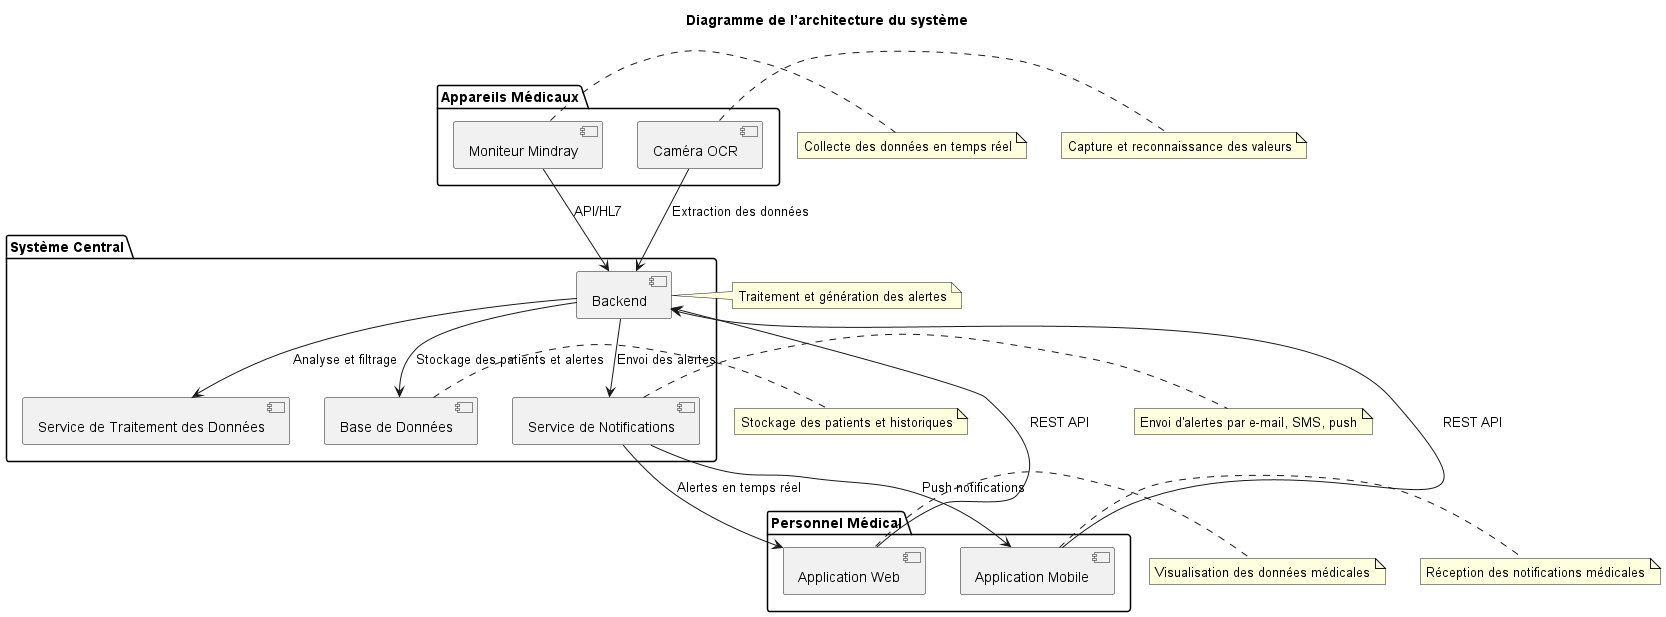
\includegraphics[width=1\textwidth]{chapter2/sections/diagrams/architecture.png}
    \caption{Diagramme de l’architecture du système}
    \label{fig:architecture}
\end{figure}
\subsection{Diagramme de déploiement}
Le diagramme de déploiement (Figure~\ref{fig:diagramme_deploiement}) illustre l’architecture du système, reliant les équipements médicaux, le backend et les interfaces utilisateur.

\begin{figure}[h]
    \centering
    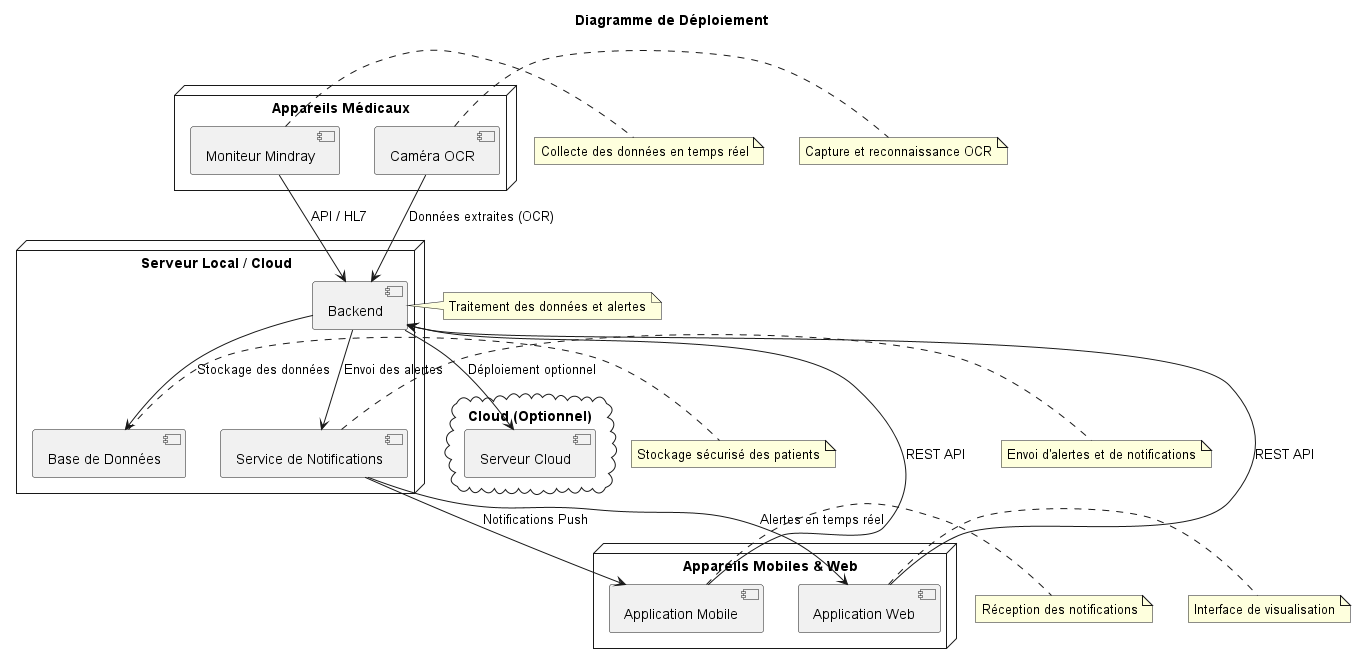
\includegraphics[width=1\textwidth]{chapter2/sections/diagrams/deployment_diagram.png}
    \caption{Diagramme de Déploiement du Système}
    \label{fig:diagramme_deploiement}
\end{figure}

\subsection{Composants et Déploiement}
\begin{itemize}
    \item \textbf{Serveur Local / Cloud} :
    \begin{itemize}
        \item \textbf{Backend} : Traitement des données et gestion des alertes.
        \item \textbf{Base de Données} : Stockage des patients et alertes.
        \item \textbf{Service de Notifications} : Envoi d’alertes (e-mails, push).
    \end{itemize}
    \item \textbf{Appareils Médicaux} :
    \begin{itemize}
        \item \textbf{Moniteur Mindray} : Envoie les données via API HL7.
        \item \textbf{Caméra OCR} : Capture et extrait les valeurs vitales.
    \end{itemize}
    \item \textbf{Applications Mobiles \& Web} :
    \begin{itemize}
        \item \textbf{Application Web / Mobile} : Consultation des données via REST API.
    \end{itemize}
\end{itemize}

\subsection{Flux de Communication}
\begin{enumerate}
    \item Collecte des données via HL7 ou OCR.
    \item Analyse et stockage par le backend.
    \item Détection des anomalies et envoi d’alertes.
    \item Consultation des alertes et données par le personnel médical.
\end{enumerate}

\subsection{Justification}
L’architecture garantit \textbf{modularité} (séparation des composants), \textbf{réactivité} (alertes en temps réel) et \textbf{interopérabilité} (compatibilité HL7 / OCR), avec une option de déploiement sur serveur local ou cloud.


